
\subsection{Definition}

A \textbf{branch-and-bound} algorithm consists of a systematic enumeration of
candidate solutions by means of state space search: the set of candidate
solutions is thought of as forming a rooted tree with the full set at the root.

\begin{itemize}
    \item Explores branches of this tree, which represent subsets of the
solution set. 
    \item Note that before enumerating the candidate solutions of a branch, the
branch is checked against upper and lower estimated bounds on the optimal
solution, and is discarded if it cannot produce a better solution than the best
one found so far by the algorithm.
\end{itemize}

\subsection{Solving the knapsack problem with B\&B}

Given the following knapsack problem :
    \begin{tabular}{cl}
        maximize & $28x_1+30x_2 +20x_3$\\
        subject to & $4x_1+6x_2 +4x_3 \leq 9$\\
                   & $x_i \in \{0, 1\} \forall i$
    \end{tabular}

\subsubsection{Relaxation}
We can choose to relax in order to reduce the search space as much as possible.

\begin{enumerate}
    \item \textbf{Capacity relaxation}: Relax on the constraint by don't
        explore branch which already violated the constraint.

        $\Rightarrow$ Cut at tree branch when 
        we have surpassed the capacity.
        \begin{center}
        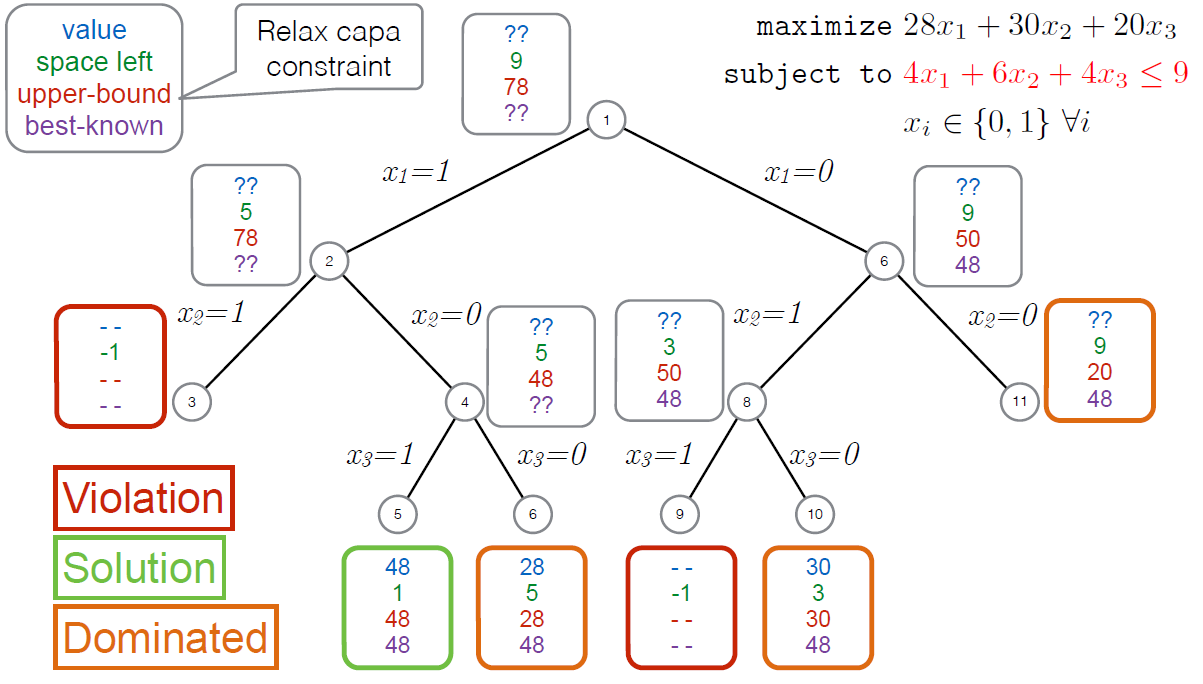
\includegraphics[width=12cm]{KnapsackBBCapaRelaxation.png}
        \end{center}
        It is far from optimal as our upper bound are not close enough to their real
        value.

    \item \textbf{Linear relaxation}: Relax on the value to maximize by
        calculating an upper bound and don't explore if the upper bound <
        actual best value.

        \paragraph{Upper bound computation}
        Given a set sorted by ratio $v_i/w_i$,
        \begin{eqnarray*}
            j &= min\{i \in I: \sum_{k \in 1,...,i} w_k > C\}\\
            UB &= \sum_{i<j} v_i + \frac{(C - \sum_{i \in 1..j-1} w_i)}{w_j} v_j
        \end{eqnarray*}

        $j$ is called the critical item which is in fact the first item (sorted by better ratio)
        which cannot be add entirely, so we just add the ratio of the item according to 
        the free space.

        \begin{center}
            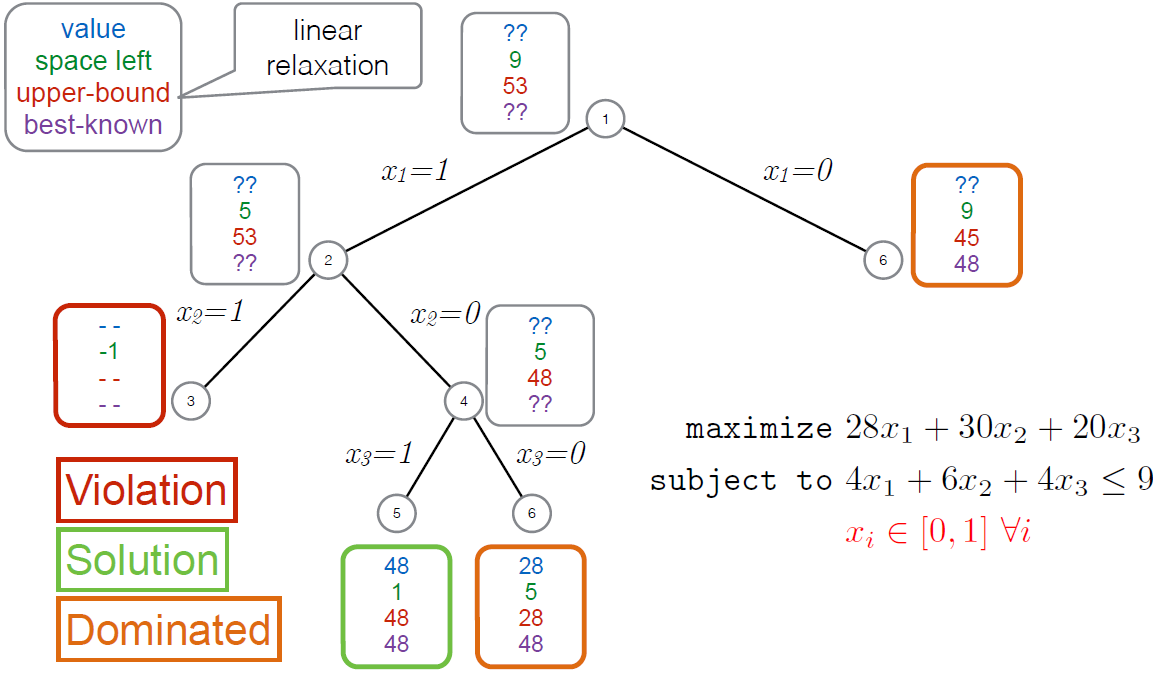
\includegraphics[width=12cm]{KnapsackBBLinearRelaxation.png}
        \end{center}

        Improving the precision of the upper-bound yields far better
        result. Take care however not to over/under estimate it (depending if you are
        on a maximisation or minimisation process) as it might prevent you to find the
        optimal solution.

\end{enumerate}


\subsection{B\&B pseudo-code}

\begin{tabular}{m{8cm}m{8cm}}
\begin{lstlisting}[mathescape, caption=BB with recursion]
def backtrackSearch(c) {
    if reject(P, c) then return
    if accept(P, c) then output(P, c)
    for s $\leftarrow$ children(c) do
        backtrackSearch(s)
}

backtrackSearch(root(P))
\end{lstlisting}
&
\begin{lstlisting}[mathescape, caption=BB with stack]
  def branchAndBound() = {
      var queue = List(root(P))

      while(queue.nonEmpty) {
          var c = queue.head
          queue = queue.tail

          if( ! reject(P, c)) {
            if( accept(P, c)) output(P, c)
            for (s $\leftarrow$ children(P, c))
            queue = s :: queue
          }
      }
  }
  \end{lstlisting}
\end{tabular}


\begin{itemize}
    \item For the knapsack, partial solution by a list of boolean: 
        $\begin{cases} 
            list[i]= 1 \text{ if item i is selected}\\
            list[i]= 0 \text{ else}\\
        \end{cases}$
\end{itemize}

\begin{center}
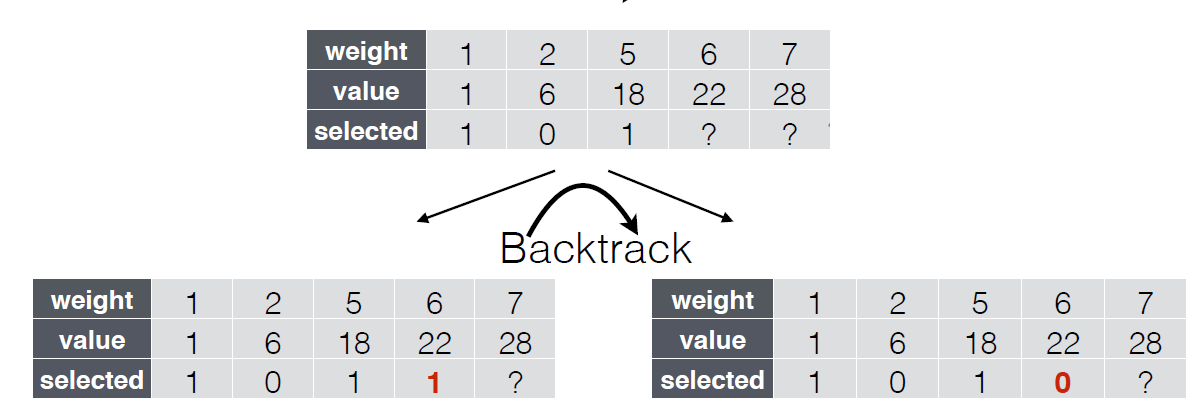
\includegraphics[width=10cm]{PartialSolBB.png}
\end{center}

\paragraph{Limitations which may affect performance}:
\begin{itemize}
    \item Must evaluate variable in the same order. We cannot affect $X_1$
        then$ X_2$ at the left side of the tree while on the other side we
        affect $X_2$ then $X_1$, each level of the tree must strictly
        correspond to the affectation of a variable.

    \item Cannot process trees which has a variable number of children easily.
        If it's the case, we could, for example, decide multiple variables at once.
\end{itemize}

\subsection{Reversible state and magical integers}

\textbf{Reversible states} are use to improve our algorithm in two way:
\begin{enumerate}
    \item By breaking the two previous limitation
    \item By use only one incremental state relative of the change
        that have been made on the parent instead of
            simply clone the parent and waste memory.
\end{enumerate}
        
\subsubsection{The idea}

To implement those reversible states, we will thus make use of three objects.

\begin{enumerate}
	\item \textbf{ReversibleContext()} : Which will be used to represent a 
	reversible state.
	\item \textbf{ReversibleInt(ReversibleContext rc, int i)} : Which will be used to 
	represent the variables of a reversible state.
	\item \textbf{TrailEntry(ReversibleInt ri, int value)} : Which will be used
	to represent changes on a stacks stocked in the context. This object will
	only be used by the ReversibleContext class.
\end{enumerate}

\begin{tabular}{m{8cm}m{7cm}}
\begin{lstlisting}[mathescape]
val rc = new ReversibleContext() 
val n1 = new ReversibleInt(rc,2)
val n2 = new ReversibleInt(rc,5) 

rc.pushState()    // Store $n_1=2$ and $n2=5$

n1.value = 6
n1.value = 5
n2.value = 4

rc.pushState()    // Store $n_1=5$ and $n2=4$

n1.value = 3
n2.value = 7

rc.pop()          // Restore $n_1=5$ and $n_2=4$
rc.pop()          // Restore $n_1=2$ and $n_2=5$
\end{lstlisting}
& 
\begin{itemize}
    \item Each reversible contains the \textbf{time} at which its last value was given
    \item A each \texttt{pushState()} the clock increase
    \item When the value of a reversible change, if its last value was given at a
        time different from the current time, then we store it before actually changing
        the current value
    \end{itemize}
\end{tabular}


\subsubsection{Push/Pop operation in reversible context}
\begin{center}
    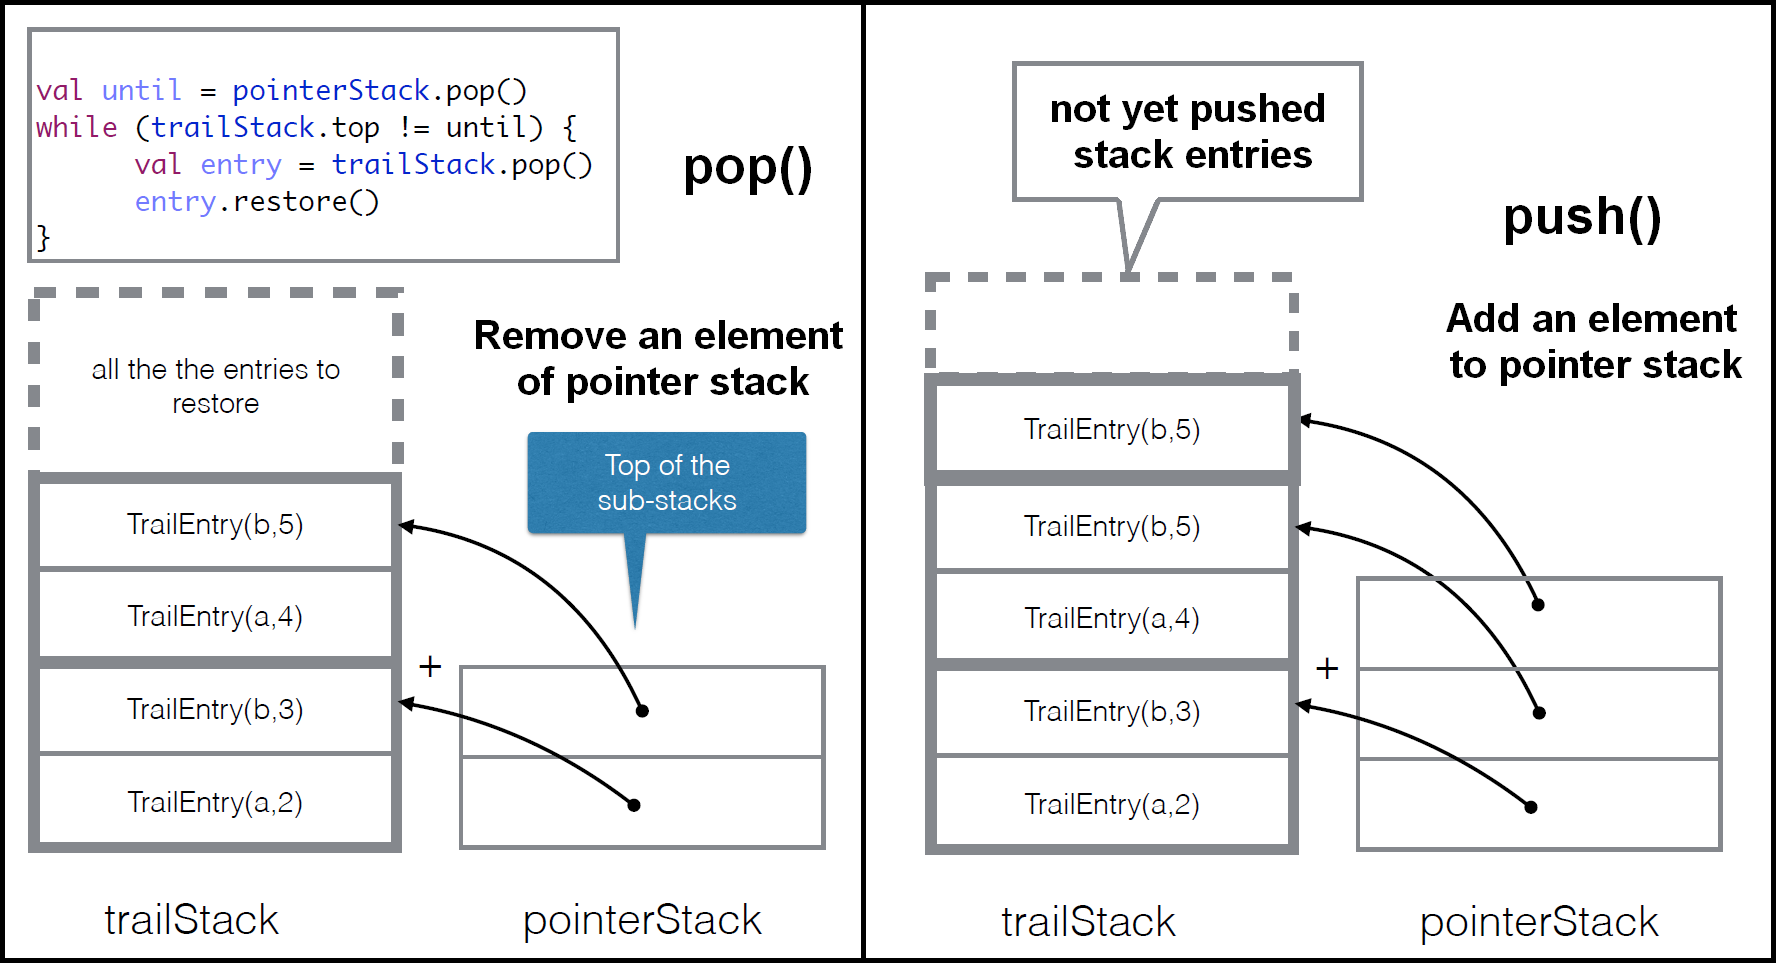
\includegraphics[width=12cm]{ReversibleStatePushPop.png}
\end{center}

\subsubsection{Implementation}

\begin{tabular}{m{8cm}m{7cm}}
\begin{lstlisting}[mathescape]
class ReversibleContext() {
    private var magicNumber: Long = 0
    private val trailStack: Stack[TrailEntry] = new Stack()
    private val pointerStack: Stack[TrailEntry] = new Stack()

    def magic: Long = magicNumber
    def pushOnTrail[T](reversible: ReversibleInt, value: Int): Unit = {
        val entry = new TrailEntry(reversible, value)
        trailStack.push(entry)
    }
    def pushState(): Unit = {
        magicNumber += 1
        pointerStack.push(trailStack.top)
    }
    def pop(): Unit = {
        restoreUntil(pointerStack.pop())
        magicNumber += 1
    }
    def restoreUntil(until: TrailEntry): Unit = {
        while (trailStack.top != until) {
            val entry = trailStack.pop()
            entry.restore()
        }
    }
}
\end{lstlisting}
& 
\begin{lstlisting}[mathescape]
class ReversibleInt(context: ReversibleContext, v: Int) {
    protected var pointer: Int = v
    private var lastMagic: Long = -1L
    trail()

    def trail(): Unit = {
        val contextMagic = context.magic
        if (lastMagic != contextMagic) {
            // Store previous value on store 
            // because magic time has changed
            lastMagic = contextMagic
            context.pushOnTrail(this, value)
        }
    }
    def value_=(value: Int): Unit = {
        if (value != pointer) {
            // Before overriding, trail it if necessary
            trail()
            this.pointer = value
        }
    }
    def value = pointer
    def restore(value: Int): Unit = pointer = value
}
\end{lstlisting}
\end{tabular}

\paragraph{Implementation B\&B using reversible}
Show example lecture 2 page 28

\subsection{Search heuristics}
With heuristic, we can at each given moment, decide what variable to instantiate 
and/or which value to assign. 

\begin{itemize}
    \item Variables heuristic: Choose which variable will know be 
        assigned
    \item Value heuristic: Choose the order of assigned value for
        the variables
    \end{itemize}

\subsubsection{Iterative Discrepancy Search}

\begin{tabular}{m{11cm}m{6cm}}
\begin{description}
    \item[Discrepancy] = Number of right (the side in a tree) decisions
\end{description}
\begin{lstlisting}[mathescape]
for (d $\leftarrow$ 0 to 100) {
    problem.search(maxDiscrepancy = d)
}
\end{lstlisting}
&
    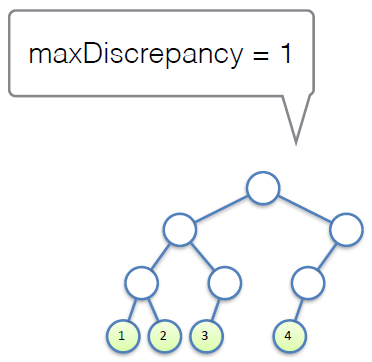
\includegraphics[width=4cm]{LimiteDiscrpancy.png}
\end{tabular}


\paragraph{Advantages}
\begin{itemize}
    \item Easy to implement, weak memory consumption (DFS)
    \item Can potentially be fast \textbf{depending on the heuristics},
        but also slower because of recomputation which are normally for the
        most part pruning in recomputation.
\end{itemize}

\textbf{If the discrepancy search does not explore the tree completely, 
it is not considered complete !} This can however be used as a form of greedy
algorithm.

\subsubsection{Best first search}

Expand the open node with the best upper-bound first (maximization) !
Although fairly efficient and easy to implement, this heuristic has two drawbacks :

\begin{enumerate}
	\item You won't have a feasible solution directly (implication for the pruning).
	\item Memory usage is difficult to control.
\end{enumerate}

\begin{figure}[!ht]
    \centering
    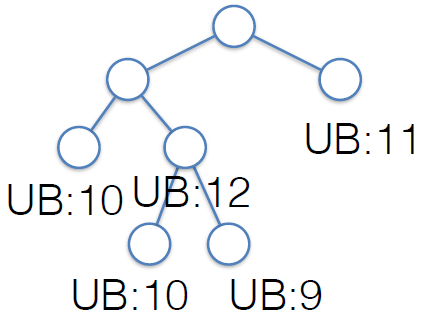
\includegraphics[width=0.3\linewidth]{BestFirstSearchBBHeuristic.png}
    \caption{Representation of the best first search heuristic}
    \label{fig:Knapsack_example}
\end{figure}
\FloatBarrier

\subsubsection{Other heuristics}

TODO

\subsection{Other B\&B optimisations}

\subsubsection{Symmetry detection}

In case of symmetric items in the knapsack set (understand identical), we can reduce the
search space significantly as the items are completely interchangeable.

\subsubsection{Dominance detection}

In case an item b is dominated by another item a
(b is dominated by a if $V_a \geq V_b \wedge W_a \leq W_b$)
It is never interesting to take b if a is not also taken ! 

$\Rightarrow$ An optimal solution cannot have a = 0 and b = 1. 
We can thus avoid to explore such states.

\subsection{Bonus questions}

\subsubsection{Reversible set}

\begin{lstlisting}
//WARNING : UNTESTED but the idea is there

//Create ReversibleSet class as follows
// 1 : Add set variable which store curent set
// 2 : Modify pointer to save multiples changes
// 3 : Add remove method which remove in set and adds to changes made
// 4 : Modify trail method to push changes one by one
// 5 : Modifify restore methode to remove unpushed changes and add back argument value
// 6 : Write the get iterator method

class ReversibleSet(context: ReversibleContext, s: Set) {
	protected var currentSet: Set = s //Set
	protected var pointer: Array<Integer> = [] //List of changes
	private var lastMagic: Long = -1L
	trail()
	
	def trail(): Unit = {
		val contextMagic = context.magic
		if (lastMagic != contextMagic) {
			//We need to push values
			lastMagic = contextMagic
			for elem in pointer{ //One push per elem removed
				context.pushOnTrail(this, elem)
			}
			pointer = [] //Reset change array since change have been pushed
		}
	}
	def remove(value: Int): Unit = {
		if (value != pointer) {
			trail() //Always call this method before making changes
			this.currentSet.remove(value) //Remove value in set
			this.pointer.add(value) //Add to changes made
		}
	}
	def getIterator() : Unit = {
		return set.iterator(); //Assuming our set implements iterable
	}
	def set = currentSet //To acces current set value
	
	def restore(value: Int): Unit = {
		//Remove unpushed changes
		for elem in value{
			set.add(elem)
		}
		//(so that we don't add multiple time in case of multiple changes)
		pointer = [] //Reinit change list 
		//Add the value in argument to the set
		set.add(value);
	}
}
\end{lstlisting}

\subsubsection{Explicit stack DFS's pseudo code}

\begin{lstlisting}
//Init stack
stack state_to_visit = new stack();
state_to_visit.add((0,initState)); 
//A tuple (current index, state where no item are taken)
//Init method variable
int maxIndex = nbVariableToAsssign - 1;
state bestSol = initState;
while(!state_to_visit.isEmpty()) {
  (index, state) = state_to_visit.pop();
  if(index > maxIndex){
  	//Computation finished, evaluate state
  	if(bestSol.value < state.value) bestSol = state;
  }
  else if(state.getUpperBound() > bestSol.value){
  	newState = state.makeCopy()
  	//Add current elem not selected state to stack
  	state_to_visit.push((index+1, state));
  	//Add current elem selected state to stack => will be visited first
  	newState.changeElemAtIndex(index, 1); //Set as taken
  	if(newState.isUnderCapacityConstraint()) state_to_visit.push((index+1, newState));
  }
}
return bestSol; 
\end{lstlisting}

\subsection{Exam}
\begin{itemize}
    \item Give the pseudo-code of a backtracking search algorithm
        \begin{itemize}
            \item  What kind of search tree exploration is it?
            \item  What are the advantages of such an exploration?
        \end{itemize}
    \item Explain the trailing and reversible mechanism
        \begin{itemize}
            \item  Sketch the code to implement it, give an example of how to use
                it
            \item  Illustrate the solving of a combinatorial problem with a
                backtracking search using reversibles to restore state
        \end{itemize}
    \item  Explain Limited Discrepancy Search, why it is useful? How to
        implement it using DFS while staying complete
    \item  Explain/Illustrate the heuristics and how it can impact B\&B
    \item  Explain what are symmetries and dominances, how to avoid
        them?
\end{itemize}
